\documentclass[11pt]{beamer}

\usetheme{Madrid}
\usecolortheme{default}

\usepackage[utf8]{inputenc}
\usepackage{amsmath, amssymb}
\usepackage{physics}
\usepackage{graphicx}
\usepackage{bm}

\title[Static Fluid Spheres in GR]{Static Solutions of Einstein's Field Equations for Spheres of Fluid and Application to massive neutron cores}
\author[R.~C.~Tolman]{Based on: R.~C.~Tolman, Phys.\ Rev.\ \textbf{55}, 364--373 (1939) and \\
Based on: J.~R.~Oppenheimer \& G.~M.~Volkoff,\\
\emph{Phys.\ Rev.} \textbf{55}, 374--381 (1939)}
\institute{Summary prepared by Gytis Vėjelis}
\date{}

\begin{document}

%--------------------------------------------------
\begin{frame}
  \titlepage
\end{frame}

%--------------------------------------------------
\begin{frame}{Goal}
  \begin{itemize}
    \item Solve Einstein's field equations for \textbf{static}, \textbf{spherically symmetric} distributions of perfect fluid.
    \item There are only a few known solutions:
      \begin{itemize}
        \item Einstein static universe (constant $\rho$, $p$ everywhere).
        \item Schwarzschild interior solution (incompressible fluid with constant $\rho$).
        \item Schwarzschild exterior solution (vacuum outside spherical body).
        \item de~Sitter solution (vacuum with cosmological constant).
      \end{itemize}
  \end{itemize}
\end{frame}  % <-- this was missing

%--------------------------------------------------
\begin{frame}{Einstein Equations and Conventions}
  \begin{itemize}
    \item Units: $c=G=1$.
    \item Einstein equations with cosmological constant $\Lambda$:
      \[
        8\pi T_{\mu\nu} = R_{\mu\nu} - \frac{1}{2} R g_{\mu\nu} + \Lambda g_{\mu\nu} .
      \]
    \item Matter: \textbf{perfect fluid}
      \[
        T^{\mu\nu} = (\rho + p) u^\mu u^\nu - p g^{\mu\nu}.
      \]
    \item We look for \textbf{static}, \textbf{spherically symmetric} configurations in \textbf{gravitational equilibrium}.
  \end{itemize}
\end{frame}

%--------------------------------------------------
\begin{frame}{From the Metric to Einstein Equations}
  \textbf{Goal:} Given a metric $g_{\mu\nu}$, compute $G_{\mu\nu}$ and solve
  \[
    G_{\mu\nu} + \Lambda g_{\mu\nu} = 8\pi T_{\mu\nu}.
  \]

  \medskip
  \textbf{1. Start with Static, spherically symmetric ansatz:}
  \[
    ds^2 = e^{\nu(r)} dt^2 - e^{\lambda(r)} dr^2 - r^2 d\Omega^2.
  \]

  \textbf{2. Christoffel symbols}
  \[
    \Gamma^\rho_{\mu\nu}
    = \frac{1}{2} g^{\rho\sigma}
    \left( \partial_\mu g_{\sigma\nu}
         + \partial_\nu g_{\sigma\mu}
         - \partial_\sigma g_{\mu\nu} \right).
  \]

  \textbf{3. Riemann tensor}
  \[
    R^\rho_{\ \sigma\mu\nu}
    = \partial_\mu \Gamma^\rho_{\nu\sigma}
    - \partial_\nu \Gamma^\rho_{\mu\sigma}
    + \Gamma^\rho_{\mu\lambda}\Gamma^\lambda_{\nu\sigma}
    - \Gamma^\rho_{\nu\lambda}\Gamma^\lambda_{\mu\sigma}.
  \]

  \textbf{4. Ricci tensor and scalar}
  \[
    R_{\mu\nu} = R^\rho_{\ \mu\rho\nu},
    \qquad
    R = g^{\mu\nu} R_{\mu\nu}.
  \]

  \textbf{5. Einstein tensor}
  \[
    G_{\mu\nu} = R_{\mu\nu}
    - \tfrac{1}{2} R g_{\mu\nu}.
  \]
\end{frame}


\begin{frame}{Perfect Fluid in the Static Frame}
  \begin{itemize}
    \item For the RHS we can consider fluids rest frame and obtain
      \[
        T^1_1 = T^2_2 = T^3_3 = -p, \qquad T^4_4 = \rho.
      \]
    \item Effectively:
          \[
      T^\mu_{\ \nu} =
      \begin{pmatrix}
      \rho & 0 & 0 & 0 \\
      0 & -p & 0 & 0 \\
      0 & 0 & -p & 0 \\
      0 & 0 & 0 & -p
      \end{pmatrix}.
      \]

  \end{itemize}
\end{frame}


%--------------------------------------------------
\begin{frame}{Reduced Field Equations}
  \small
  Using Tolman’s notation the field equations reduce to
  \begin{align*}
    8\pi \rho &= e^{-\lambda} \left(\frac{\lambda'}{r} - \frac{1}{r^2}\right) + \frac{1}{r^2} + \Lambda, \\
    8\pi p &= e^{-\lambda} \left(\frac{\nu'}{r} + \frac{1}{r^2}\right) - \frac{1}{r^2} + \Lambda, \\
    8\pi p &= e^{-\lambda} \left(
      \frac{\nu''}{2} - \frac{\lambda' \nu'}{4}
      + \frac{\nu'^2}{4} + \frac{\nu' - \lambda'}{2r}
    \right) + \Lambda .
  \end{align*}
  \begin{itemize}
    \item Two equations for $p$ must be equal $\Rightarrow$ one relation between $\lambda$ and $\nu$.
    \item Together: three ODEs for four unknowns ($\lambda (r)$, $\nu (r)$, $\rho (r)$, $p (r)$).
  \end{itemize}
\end{frame}


%--------------------------------------------------
\begin{frame}{Tolamn's Idea}
  \begin{itemize}
    \item Mathematically, we need \textbf{one more relation} to close the system. One approach would be to consider some physical choice: \textbf{equation of state} $p=p(\rho)$. But this typically leads to non–elementary ODEs needing numerical integration.

    \item Tolman’s idea:
        Impose a relation between the metric functions $\lambda(r)$ and $\nu(r)$ that makes the system integrable. Consider the physics later
  \end{itemize}
\end{frame}


\begin{frame}{Rewriting the main equation}
  
  \begin{itemize}
      \item Toleman rewrites the equations into \textbf{almost} integrable form:
        \begin{align*}
          \frac{d}{dr}\!\left( \frac{e^{-\lambda} - 1}{r^2} \right)
          + \frac{d}{dr}\!\left( \frac{e^{-\lambda} \nu'}{2r} \right)
          + e^{-\lambda - \nu} \frac{d}{dr}\!\left( \frac{e^{\nu} \nu'}{2r} \right)
          = 0
          \\
          8\pi p
          = e^{-\lambda} \!\left( \frac{\nu'}{r} + \frac{1}{r^2} \right)
          - \frac{1}{r^2} + \Lambda
          \\
          8\pi \rho
          = e^{-\lambda} \!\left( \frac{\lambda'}{r} - \frac{1}{r^2} \right)
          + \frac{1}{r^2} - \Lambda
        \end{align*}
      \item Then get solutions by:
      \begin{enumerate}
        \item Choose an \textbf{ansatz} relating $\lambda$ and $\nu$.
        \item Integrate the resulting equation for the metric.
        \item Use remaining Einstein equations to find $\rho(r)$ and $p(r)$.
      \end{enumerate}
    \end{itemize}
\end{frame}

\begin{frame}{Solutions I–VIII}
  \small
  Tolman lists eight families of solutions, labeled I–VIII:
  \begin{description}
    \item[Solution I] Einstein static universe: $e^\nu = \text{const}$, spatial curvature radius $R$.
    \item[Solution II] Schwarzschild–de~Sitter: constant $e^\lambda$, includes mass $m$ and $\Lambda$.
    \item[Solution III] Schwarzschild interior: incompressible fluid, constant density $\rho$.
    \item[Solution IV] New compressible-fluid model:
      \[
        e^\lambda = \frac{1+2r^2/A^2}{1-r^2/R^2},\quad e^\nu = B^2(1+r^2/A^2)
      \]
      with $\rho(r)$ and $p(r)$ finite at $r=0$.
    \item[Solution V] Family with $e^\nu \propto r^{2n}$, $e^{-\lambda} = 1 - (1+2n-n^2)(r/R)^2$.
    \item[Solution VI] Another family with $e^{-\lambda} = \text{const}$ and power-law $r$-dependence in $e^\nu$.
    \item[Solution VII] More complicated polynomial/reciprocal form (less convenient physically).
    \item[Solution VIII] More general power–law ansatz, including II as a special case.
  \end{description}
\end{frame}

\begin{frame}{Birkhoff's Theorem}

\begin{block}{Birkhoff's Theorem}
Any spherically symmetric solution of the vacuum Einstein equations must be \emph{static} and
is uniquely given by the Schwarzschild--(de~Sitter) metric.
\end{block}

\medskip

\begin{itemize}
    \item The external gravitational field of any spherically symmetric
          object (star, planet, collapsing matter) is \emph{static}
          regardless of time-dependent interior dynamics.
    \item The vacuum exterior is always described by:
    \[
    ds^2 = 
    \left(1 - \frac{2M}{r} - \frac{\Lambda r^2}{3}\right) dt^2
    \;-\;
    \frac{dr^2}{\,1 - \frac{2M}{r} - \frac{\Lambda r^2}{3}}
    \;-\; r^2 d\Omega^2 .
    \]
    \item Mass parameter \(M\) fully characterizes the exterior geometry.
\end{itemize}
\end{frame}


\begin{frame}{Physical Fluid Spheres and Matching}
  \begin{itemize}
    \item Physical model: finite fluid sphere ($0 \le r \le r_b$) surrounded by vacuum ($r > r_b$).
    \item Inside: one of Tolman’s interior solutions with $p(r_b)=0$, $\rho(r_b) > 0$.
    \item Outside: Schwarzschild metric (neglect $\Lambda$ on stellar scales)
      \[
        ds^2 = -\left(1-\frac{2m}{r}\right)^{-1} dr^2 - r^2 d\Omega^2
        + \left(1-\frac{2m}{r}\right)dt^2,
      \]
      where $m$ is the gravitational mass seen at infinity.
    \item At $r=r_b$, require continuity of the metric and vanishing pressure:
    \[
    \begin{alignedat}{2}
    p(r_b) &= 0, \qquad
    e^{\nu(r_b)} &= 1 - \frac{2m}{r_b}, \qquad
    e^{-\lambda(r_b)} &= 1 - \frac{2m}{r_b}.
    \end{alignedat}
    \]
  \end{itemize}
\end{frame}

\begin{frame}{Solution IV: Metric, Density, Pressure, Equation of State}
  \small
  \begin{itemize}
    \item Ansatz: $e^{\nu/2} r^{-1} = \text{const}$ $\Rightarrow$ $e^{\nu/2} \propto r$ (Tolman’s relation).
    \item Resulting interior metric:
      \[
        ds^2 = -\frac{1+2r^2/A^2}{1-r^2/R^2} \, dr^2
               - r^2 d\theta^2 - r^2 \sin^2\theta\, d\phi^2
               + B^2 \left(1+\frac{r^2}{A^2}\right) dt^2 .
      \]

    \item Energy density and pressure (for $\Lambda=0$):
      \[
        8\pi \rho(r) = \frac{1}{A^2} + \frac{3}{R^2}
                       - \frac{1}{A^2} \frac{1+3r^2/R^2}{1+2r^2/A^2},
      \quad 
        8\pi p(r) = \frac{1}{A^2} - \frac{1}{R^2}
                    - \frac{1}{A^2}\frac{1-r^2/R^2}{1+2r^2/A^2}.
      \]
    \item Central values ($r=0$):
      \[
        8\pi \rho_c = \frac{3}{R^2} + \frac{1}{A^2}, \qquad
        8\pi p_c     = \frac{1}{A^2} - \frac{1}{R^2}.
      \]
    \item Equation of state can be written in a simple quadratic form:
      \[
        ( \rho - \rho_c )^2
         = \rho_c^2 + 6 (\rho_c - p_c)(p_c - p) + 9 (p_c - p)^2 .
      \]
      (Here $A$ and $B$ are integration constants)
  \end{itemize}
\end{frame}

%--------------------------------------------------
\begin{frame}{Solution IV: Physical Features}
  \small
  \begin{itemize}
    \item Parameters $A, R$ control central density/pressure and size.
    \item For $R^2 > A^2$, pressure and density decrease monotonically with $r$.
    \item Pressure vanishes at $r=r_b$:
      \[
        r_b = R \sqrt{1 - \frac{A^2}{R^2}} ,
      \]
      giving a finite radius.
    \item Density at boundary remains positive.
    \item Ratio $p/\rho$ never exceeds $1/3$ if $R^2 \gtrsim 11.5\, A^2$ (Tolman’s estimate).
    \item As $A,R\to\infty$, star radius grows and central density/pressure go to zero.
  \end{itemize}
\end{frame}

%==================================================
\section{Examples: Solutions V and VI (Special Cases)}

%--------------------------------------------------
\begin{frame}{Solution V: $n=-\tfrac{1}{2}$ Case}
  \small
  \begin{itemize}
    \item Take the family with
      \[
        e^{-\lambda} = 1 - (1+2n-n^2)\left(\frac{r}{R}\right)^2,
        \qquad e^{\nu/2} \propto r^n .
      \]
    \item Special choice $n=-\tfrac{1}{2}$:
      \begin{itemize}
        \item Central pressure and density $\to \infty$.
        \item Ratio at the center:
          \[
            \frac{p_c}{\rho_c} = \frac{1}{3},
          \]
          characteristic of radiation or ultrarelativistic matter.
      \end{itemize}
    \item Pressure decreases to zero at a finite radius $r_b$, while density stays finite there.
    \item Useful toy model for extremely compact objects with radiation-dominated core.
  \end{itemize}
\end{frame}

%--------------------------------------------------
\begin{frame}{Solution VI: $n=-\tfrac{1}{2}$ and Blackbody Limit}
  \small
  \begin{itemize}
    \item Another family with $e^{-\lambda} = \text{const}$ and power–law behavior in $e^\nu$.
    \item Again, a special choice $n=-\tfrac{1}{2}$ gives $p_c/\rho_c = 1/3$.
    \item Equation of state at high density:
      \[
        p - \frac{1}{3}\rho \approx \text{const}\times \rho^{2/3},
      \]
      resembling a highly degenerate Fermi gas at large $\rho$.
    \item As certain parameter ratios $\to 0$, the solution approaches a limiting
      \emph{blackbody radiation solution} with $p=\rho/3$ throughout.
    \item Tolman notes close relation to Oppenheimer–Volkoff neutron star models.
  \end{itemize}
\end{frame}

\begin{frame}{Motivation: Beyond Tolman's Analytic Interiors}
  \begin{itemize}
    \item Tolman classified analytic interior solutions, but realistic stars obey a \emph{physical equation of state}.
    \item After nuclear fuel is exhausted, stellar cores may become extremely dense.
    \item At high densities electrons combine with protons $\Rightarrow$ degenerate \textbf{neutron matter}.
    \item Oppenheimer \& Volkoff (1939) study:
      \begin{itemize}
        \item General relativistic hydrostatic equilibrium (TOV equation).
        \item Equation of state of a cold, degenerate Fermi gas of neutrons.
        \item Existence of a maximum mass for static neutron cores.
      \end{itemize}
  \end{itemize}
\end{frame}

\begin{frame}{General Relativistic Hydrostatic Equilibrium}
  Starting from the spherically symmetric metric and perfect fluid:
  \[
    ds^2 = e^{\nu(r)} dt^2 - e^{\lambda(r)} dr^2 - r^2 d\Omega^2 ,
  \]
  and energy–momentum conservation, Oppenheimer \& Volkoff derive the
  \textbf{TOV equation}:
  \[
    \frac{dp}{dr}
    = -\frac{(\rho + p)\,\big[m(r) + 4\pi r^3 p\big]}
            {r\,[r - 2m(r)]},
  \]
  \begin{itemize}
    \item This is the relativistic generalization of hydrostatic equilibrium.
    \item Much stronger gravitational effects arise when $r \to 2m(r)$.
  \end{itemize}
\end{frame}

\begin{frame}{Equation of State: Cold Degenerate Neutron Gas}
  \small
  Oppenheimer \& Volkoff use the exact Fermi–gas equation of state
  (parametrized by $t$):
  \[
    \rho = K(\sinh t - t), \qquad
    p = \frac{K}{3}\left(\sinh t - 8 \sinh\frac{t}{2} + 3t\right),
  \]
  with
  \[
    K = \frac{m_n^4 c^5}{4\pi^2\hbar^3}. \quad \text{and} \quad t = 4 \log \left( \frac{\hat{p}}{\mu_0 c} + \left[ 1 + \frac{\hat{p}}{\mu_0 c} \right] \right)
  \]
  \begin{itemize}
    \item At low density ($t \ll 1$): Newtonian polytrope $p \propto \rho^{5/3}$.
    \item At extremely high density ($t \to \infty$):
      \[
        p \to \frac{1}{3}\rho,
      \]
      the \textbf{ultrarelativistic limit}.
    \item The EOS becomes stiff but not stiff enough to support arbitrarily large masses.
  \end{itemize}
\end{frame}

\begin{frame}{Solving the Structure Equations}
  \begin{itemize}
    \item Choose a central value $t_0$ (equivalently $\rho_c$).
    \item Integrate numerically:
      \begin{align*}
        \frac{dm}{dr} &= r^2 (\sinh t - t) \\
        \frac{dt}{dr} &= - \frac{4}{r(r-2m)} \frac{\sinh t - 2 \sinh \dfrac{1}{2} t}{\cosh t - 4 \cosh \dfrac{1}{2} t + 3} \times [\frac{1}{2} r^3 (\sinh t + 8 \sinh \frac{1}{2} t + 3t) + u]
      \end{align*}
      until $p(r_b) = 0$.
    \item This determines the stellar radius $r_b$ and the total gravitational mass $M = m(r_b)$.

    \item Repeat for many $t_0$ to obtain $M(t_0)$.
  \end{itemize}
\end{frame}



\begin{frame}
\centering
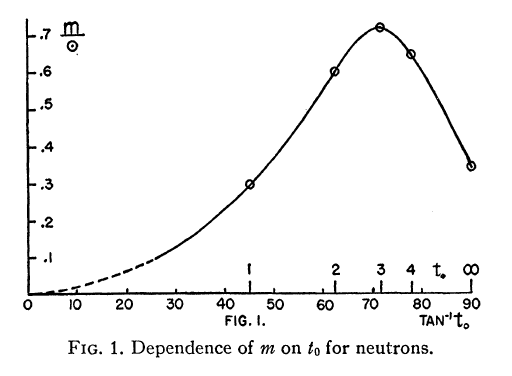
\includegraphics[width=0.45\textwidth]{image1.png}
\hfill
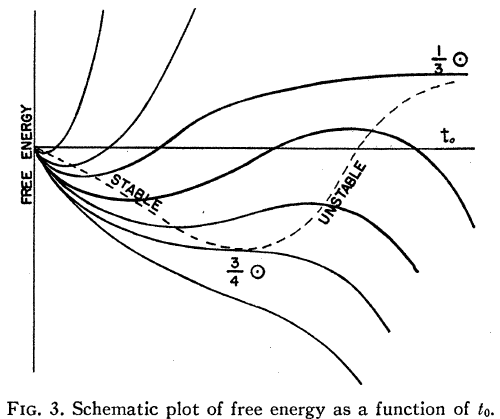
\includegraphics[width=0.45\textwidth]{image3.png}
\end{frame}


\begin{frame}{The Oppenheimer-Volkoff Limit}
  \begin{itemize}
    \item Numerical integration shows:
      \[
        M_{\mathrm{max}} \approx 0.7\, M_\odot
      \]
      for a cold neutron gas (Fermi EOS).
    \item For $M > M_{\mathrm{max}}$:
      \begin{itemize}
        \item No static solutions.
        \item Pressure cannot balance gravity.
        \item The core must collapse indefinitely (GR effect).
      \end{itemize}
    \item The limiting configuration is \textbf{not} singular in $g_{\mu\nu}$:
      GR effects dominate before an event horizon forms.
  \end{itemize}

\end{frame}


\begin{frame}{Physical Interpretation}
  \begin{itemize}
    \item At low density: pressure dominated by nonrelativistic neutron degeneracy.
    \item At high density: neutrons become ultrarelativistic, $p \simeq \rho/3$.
    \item But relativity strengthens gravity so pressure gravitates
    \item Pressure grows more slowly than gravity at high density.
    \item No equation of state of the form $p \le \rho/3$ can support arbitrarily large mass.
  \end{itemize}
\end{frame}

\begin{frame}{Relation to Tolman's Solutions}
  \small
  Oppenheimer \& Volkoff explicitly compare their results with Tolman's
  analytic classes to understand limiting behavior.
  \begin{itemize}
    \item \textbf{Tolman IV}: finite central pressure, realistic density profiles.
      \begin{itemize}
        \item Exhibits a maximum mass for given central values.
        \item Qualitatively reproduces the OV limit.
      \end{itemize}
    \item \textbf{Tolman V and VI}: singular or ultrarelativistic solutions.
      \begin{itemize}
        \item Approach $p = \rho/3$ at high density.
        \item Mirror the behavior near the OV maximum where core becomes radiation-like.
      \end{itemize}
  \end{itemize}

  \medskip
  These analytic families help interpret why neutron stars have a maximum mass.
\end{frame}

\begin{frame}{Astrophysical Implications}
  \begin{itemize}
    \item Ordinary stars, after exhausting nuclear fuel, may form neutron cores.
    \item But:
      \[
        M_{\mathrm{core}} > 0.7 M_\odot \quad \Rightarrow \quad \text{no static equilibrium}.
      \]
    \item Therefore massive stars cannot end as static neutron cores.
    \item They must undergo continued collapse.
    \item Now we know that this is the formation of black holes
  \end{itemize}
\end{frame}

\begin{frame}
  \LARGE
  \center
  Thank you
\end{frame}

\end{document}
